\documentclass{beamer}
\usepackage[utf8]{inputenc}

\usetheme{Madrid}
\usecolortheme{default}
\usepackage{amsmath,amssymb,amsfonts,amsthm}
\usepackage{txfonts}
\usepackage{tkz-euclide}
\usepackage{listings}
\usepackage{adjustbox}
\usepackage{array}
\usepackage{tabularx}
\usepackage{gvv}
\usepackage{lmodern}
\usepackage{circuitikz}
\usepackage{tikz}
\usepackage{graphicx}
\usepackage{mathtools}

\setbeamertemplate{page number in head/foot}[totalframenumber]

\usepackage{tcolorbox}
\tcbuselibrary{minted,breakable,xparse,skins}



\definecolor{bg}{gray}{0.95}
\DeclareTCBListing{mintedbox}{O{}m!O{}}{%
  breakable=true,
  listing engine=minted,
  listing only,
  minted language=#2,
  minted style=default,
  minted options={%
    linenos,
    gobble=0,
    breaklines=true,
    breakafter=,,
    fontsize=\small,
    numbersep=8pt,
    #1},
  boxsep=0pt,
  left skip=0pt,
  right skip=0pt,
  left=25pt,
  right=0pt,
  top=3pt,
  bottom=3pt,
  arc=5pt,
  leftrule=0pt,
  rightrule=0pt,
  bottomrule=2pt,
  toprule=2pt,
  colback=bg,
  colframe=orange!70,
  enhanced,
  overlay={%
    \begin{tcbclipinterior}
    \fill[orange!20!white] (frame.south west) rectangle ([xshift=20pt]frame.north west);
    \end{tcbclipinterior}},
  #3,
}
\lstset{
    language=C,
    basicstyle=\ttfamily\small,
    keywordstyle=\color{blue},
    stringstyle=\color{orange},
    commentstyle=\color{green!60!black},
    numbers=left,
    numberstyle=\tiny\color{gray},
    breaklines=true,
    showstringspaces=false,
}
\title{9.5.9}
\date{30th September, 2025}
\author{Puni Aditya - EE25BTECH11046}

\begin{document}

\frame{\titlepage}
\begin{frame}{Question}
Find the value of p for which one root of the quadratic equation 
\begin{align*}
    px^2 - 14x + 8 = 0
\end{align*}
is 6 times the other.

\end{frame}

\begin{frame}{Theoretical Solution}
\begin{align*}
    g\brak{\vec{x}} = \vec{x}^\top\vec{V}\vec{x} + 2\vec{u}^\top\vec{x} + f = 0 \\
    \vec{x} = \vec{h} + \kappa\vec{m}
\end{align*}
\begin{align}
    \kappa_{1,2} = \frac{-\vec{m}^\top\brak{\vec{V}\vec{h}+\vec{u}} \pm \sqrt{\brak{\vec{m}^\top\brak{\vec{V}\vec{h}+\vec{u}}}^2 - \brak{\vec{m}^\top\vec{V}\vec{m}}g\brak{\vec{h}}}}{\vec{m}^\top\vec{V}\vec{m}}
\end{align}
\end{frame}

\begin{frame}{Theoretical Solution}
\begin{align*}
    \text{Parabola: } &px^2 - 14x - y + 8 = 0 \\
    \text{Line: } &\vec{e_2}^\top\vec{x} = 0
\end{align*}
\begin{align}
    \vec{V} = \myvec{p & 0 \\ 0 & 0}, \text{ } \vec{u} = \myvec{-7 \\ -1/2}, \text{ } f = 8
\end{align}
\begin{align}
    \vec{x} = \kappa\vec{e_1} \implies \vec{h} = \vec{0}, \text{ } \vec{m} = \vec{e_1}
\end{align}
\begin{align}
    \vec{m}^\top\vec{V}\vec{m} &= \vec{e_1}^\top\vec{V}\vec{e_1} = p \\
    \vec{m}^\top\brak{\vec{V}\vec{h} + \vec{u}} &= \vec{e_1}^\top\vec{u} = -7 \\
    g\brak{\vec{h}} &= g\brak{\vec{0}} = 8
\end{align}
\end{frame}

\begin{frame}{Theoretical Solution}
\begin{align}
    \kappa_{1,2} = \frac{-\brak{-7} \pm \sqrt{\brak{-7}^2 - \brak{p}\brak{8}}}{p} = \frac{7 \pm \sqrt{49-8p}}{p}
\end{align} 
Let the intersection points be $\vec{x_1} = \kappa_1\vec{e_1}$ and $\vec{x_2} = \kappa_2\vec{e_1}$.
The condition that one root is 6 times the other means one intersection point's position vector is 6 times the other's.
\begin{align}
    \vec{x_2} &= 6\vec{x_1} \\
    \kappa_2\vec{e_1} &= 6\brak{\kappa_1\vec{e_1}} \\
    \brak{\kappa_2 - 6\kappa_1}\vec{e_1} &= \vec{0} \implies \kappa_2 = 6\kappa_1
\end{align}
\end{frame}

\begin{frame}{Theoretical Solution}
\begin{align}
    \frac{7 + \sqrt{49-8p}}{p} &= 6\brak{\frac{7 - \sqrt{49-8p}}{p}} \\
    7 + \sqrt{49-8p} &= 42 - 6\sqrt{49-8p} \\
    7\sqrt{49-8p} &= 35 \\
    \sqrt{49-8p} &= 5 \\
    49-8p &= 25 \\
    24 &= 8p \\
    p &= 3
\end{align}
\end{frame}

\begin{frame}{Plot}
\begin{figure}
	\centering
	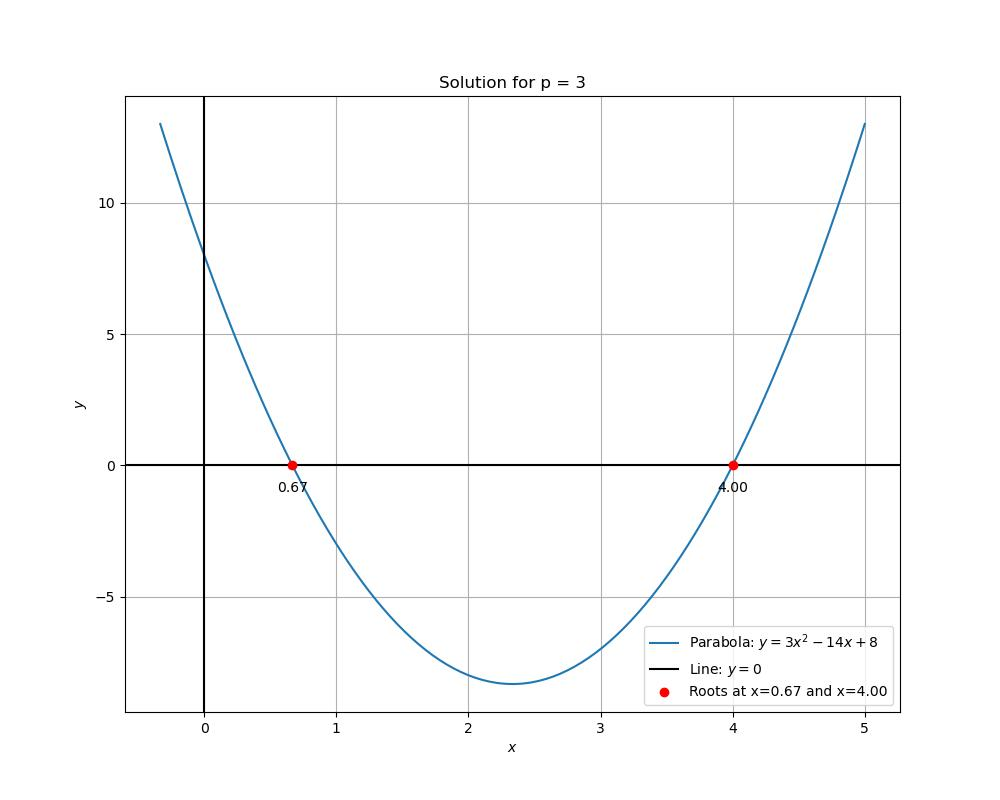
\includegraphics[width=0.5\columnwidth]{../figs/plot_c.jpg}
	\caption{Plot}
	\label{fig:fig}
\end{figure}
\end{frame}

\end{document}
